\chapter{Linear Programming}
\lecture{24}{Jun 2.}{}
\paragraph{Coloring problem}
Recall that in the graph coloring problem, we assign to vertices \(\varphi (v) \in [k]\) s.t. adjacent vertices different colors, and use as few colors as possible. Equivalently, use as few independent sets as possible to cover all vertices. 

Let \(I(G) = \left\{ \text{all independent sets in } G  \right\} \). For each \(I \in I(G)\), let 
\[
    x_I = \begin{dcases}
        1, &\text{ if we use } I \text{ in our cover}  ;\\
        0, &\text{ if we don't} .
    \end{dcases}
\] 
To cover a vertex \(v\), we need \(x_I = 1\) for some \(I\) contains \(v\). Then, the number of independent sets in our cover is 
\[
    \sum_{I \in I(G)} x_I. 
\]     
Thus we can formulate coloring problem:
\[
    \begin{aligned}
        \min~ & \sum_{I \in I(G)} x_I   \\
          \text{subject to }   &  \forall v \in V(G), \quad x_I = 1 \text{ for some } I \text{ contains v} \\
            & \forall I \in I(G), x_I \in \left\{ 0, 1 \right\}.
    \end{aligned}
\]

\paragraph{Network flow problem}
Given \((\vv{D}, s, t, c)\), the variables are \(f(\vv{e}) \quad \forall \vv{e} \in E(\vv{D})\). Our goal is to maximize flows into sink 
\[
    \sum_{\vv{e} = (v, t)} f(\vv{e}) - \sum_{\vv{e} = (t, u)} f(\vv{e}).  
\]  
The constraints are 
\begin{itemize}
    \item \(\forall \vv{e}\), \(0 \le f(\vv{e}) \le c(\vv{e})\). 
    \item \(\forall v \neq s, t\), \(\sum_{\vv{e} = (u, v)} f(\vv{e}) = \sum_{\vv{e} = (v, u)} f(\vv{e}) \).     
\end{itemize}

Thus, we can formulate this problem as 
\[
    \begin{aligned}
        \max~ & \sum_{\vv{e} = (v, t)} f(\vv{e}) - \sum_{\vv{e} = (t, v)} f(\vv{e})    \\
           \text{subject to }  & 0 \le f(\vv{e}) \le c(\vv{e}) \quad \forall \vv{e} \in E(\vv{D})  \\
            & \sum_{\vv{e} = (u, v)} f(\vv{e}) - \sum_{\vv{e} = (v, u)} f(\vv{e}) = 0 \quad \forall v \in V \text{ s.t. } v \neq s, t.  
    \end{aligned}
\]

So the example of linear programming will be max/min (linear combination of variables) subject to (inequalities involving linear combinations)

\begin{eg}
    Solve these linear programs:
    \begin{enumerate}[(i)]
        \item 
        \[
            \begin{aligned}
                \max~ &  x_1 + x_2 \\
                  \text{subject to }   & -x_1 + x_2 \ge -2  \\
                    & -3 x_1 + 2 x_2 \le 2 \\
                    &x_1 + 2 x_2 \le 4 \\
                    &x_1, x_2 \ge 0.
            \end{aligned}
        \]
        \item maximize \(2 x_1 + 4 x_2\) subject to the constraints in (i).
        \item 
        \[
            \begin{aligned}
                \max~ & x_1 + x_2  \\
                   \text{subject to }  & -x_1 + x_2 \ge 2  \\
                    & -3 x_1 + 2 x_2 \le 2 \\
                    & x_1 + 2 x_2 \le 4 \\
                    & x_1, x_2 \ge 0.
            \end{aligned}
        \]
        \item 
        \[
            \begin{aligned}
                \max~ & x_1 + x_2  \\
                  \text{subject to } & -x_1 + x_2 \ge -2  \\
                    & -3 x_1 + 2 x_2 \le 2 \\
                    & x_1, x_2 \ge 0.
            \end{aligned}
        \]
        \item
        \[
            \begin{aligned}
                \max~ & x_1 - 2 x_2  \\
                    \text{subject to } & -x_1 + x_2 \ge -2  \\
                    & -3 x_1 + 2 x_2 \le 2 \\
                    & x_1, x_2 \ge 0.
            \end{aligned}
        \]


    \end{enumerate}
\end{eg}
\begin{explanation}
The optimal of an LP over a bounded feasible region is attained at a vertex.
Label the boundary lines
\(C_1\colon x_2=x_1-2\), \(C_2\colon x_2=\tfrac{3x_1+2}{2}\), \(C_3\colon x_1+2x_2=4\).

\begin{enumerate}[(i)]

\item The feasible region (blue) has five vertices; evaluating \(x_1+x_2\):
\[
  (0,0)\mapsto 0,\quad
  (2,0)\mapsto 2,\quad
  \bigl(\tfrac{8}{3},\tfrac{2}{3}\bigr)\mapsto \tfrac{10}{3},\quad
  \bigl(\tfrac{1}{2},\tfrac{7}{4}\bigr)\mapsto \tfrac{9}{4},\quad
  (0,1)\mapsto 1.
\]
Maximum $= \boldsymbol{10/3}$ at $\bigl(\tfrac{8}{3},\tfrac{2}{3}\bigr)$ (\(\bigstar\)).

\begin{center}
\begin{tikzpicture}[scale=1.55]
  \begin{scope}
    \clip (-0.25,-0.25) rectangle (3.5,2.5);
    \fill[NavyBlue!18] (0,0)--(2,0)--({8/3},{2/3})--(0.5,1.75)--(0,1)--cycle;
    \draw[red!70!black,thick] (0,-2)--(6,4);
    \draw[ForestGreen!80!black,thick] (0,1)--(2,4);
    \draw[RawSienna!80!black,thick] (0,2)--(4,0);
  \end{scope}
  \draw[->](-0.25,0)--(3.5,0)node[right]{$x_1$};
  \draw[->](0,-0.25)--(0,2.5)node[above]{$x_2$};
  \foreach \x in {1,2,3}\draw(\x,.05)--(\x,-.05)node[below,font=\tiny]{$\x$};
  \foreach \y in {1,2}\draw(.05,\y)--(-.05,\y)node[left,font=\tiny]{$\y$};
  \fill(0,0)circle(1.5pt)node[below left,font=\tiny]{$O$};
  \fill(2,0)circle(1.5pt)node[below,font=\tiny]{$(2,0)$};
  \fill(0.5,1.75)circle(1.5pt)node[left,font=\tiny]{$\!\bigl(\tfrac{1}{2},\tfrac{7}{4}\bigr)$};
  \fill(0,1)circle(1.5pt)node[left,font=\tiny]{$(0,1)$};
  \fill[orange!90!black]({8/3},{2/3})circle(2.5pt)
      node[above right,font=\tiny]{$\bigl(\tfrac{8}{3},\tfrac{2}{3}\bigr)\;\bigstar$};
  \node[red!70!black,font=\tiny]at(3.1,1.0){$C_1$};
  \node[ForestGreen!80!black,font=\tiny]at(0.58,2.2){$C_2$};
  \node[RawSienna!80!black,font=\tiny]at(2.6,0.78){$C_3$};
\end{tikzpicture}
\end{center}

\item Same feasible region. Evaluating \(2x_1+4x_2\):
\[
  (0,0)\mapsto 0,\quad (2,0)\mapsto 4,\quad
  \bigl(\tfrac{8}{3},\tfrac{2}{3}\bigr)\mapsto 8,\quad
  \bigl(\tfrac{1}{2},\tfrac{7}{4}\bigr)\mapsto 8,\quad (0,1)\mapsto 4.
\]
Both endpoints of edge $C_3$ attain value $8$, so the maximum $= \boldsymbol{8}$ is achieved along the entire highlighted edge.

\begin{center}
\begin{tikzpicture}[scale=1.55]
  \begin{scope}
    \clip (-0.25,-0.25) rectangle (3.5,2.5);
    \fill[NavyBlue!18] (0,0)--(2,0)--({8/3},{2/3})--(0.5,1.75)--(0,1)--cycle;
    \draw[orange,line width=4pt,opacity=0.55]({8/3},{2/3})--(0.5,1.75);
    \draw[red!70!black,thick] (0,-2)--(6,4);
    \draw[ForestGreen!80!black,thick] (0,1)--(2,4);
    \draw[RawSienna!80!black,thick] (0,2)--(4,0);
  \end{scope}
  \draw[->](-0.25,0)--(3.5,0)node[right]{$x_1$};
  \draw[->](0,-0.25)--(0,2.5)node[above]{$x_2$};
  \foreach \x in {1,2,3}\draw(\x,.05)--(\x,-.05)node[below,font=\tiny]{$\x$};
  \foreach \y in {1,2}\draw(.05,\y)--(-.05,\y)node[left,font=\tiny]{$\y$};
  \fill(0,0)circle(1.5pt)node[below left,font=\tiny]{$O$};
  \fill(2,0)circle(1.5pt)node[below,font=\tiny]{$(2,0)$};
  \fill[orange!90!black](0.5,1.75)circle(2.5pt)
      node[left,font=\tiny]{$\bigl(\tfrac{1}{2},\tfrac{7}{4}\bigr)$};
  \fill(0,1)circle(1.5pt)node[left,font=\tiny]{$(0,1)$};
  \fill[orange!90!black]({8/3},{2/3})circle(2.5pt)
      node[above right,font=\tiny]{$\bigl(\tfrac{8}{3},\tfrac{2}{3}\bigr)$};
  \node[red!70!black,font=\tiny]at(3.1,1.0){$C_1$};
  \node[ForestGreen!80!black,font=\tiny]at(0.58,2.2){$C_2$};
  \node[RawSienna!80!black,font=\tiny]at(2.6,0.78){$C_3$};
  \node[orange!80!black,font=\tiny]at(1.7,1.45){optimal edge};
\end{tikzpicture}
\end{center}

\item Constraint (1) becomes $C_1'\colon x_2\ge x_1+2$. Since $x_1\ge0$ this forces $x_2\ge2$;
$C_3$ then gives $x_1+2x_2\le4\Rightarrow x_1\le0$, so the only candidate is $(0,2)$.
But $(0,2)$ violates $C_2$ (gives $4>2$). \textbf{Infeasible} — the two shaded regions are disjoint.

\begin{center}
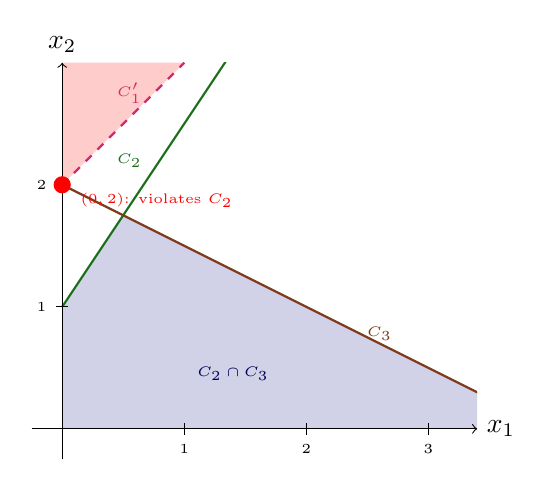
\begin{tikzpicture}[scale=1.55]
  \begin{scope}
    \clip (-0.25,-0.25) rectangle (3.4,3.0);
    % Region C2 ∩ C3 ∩ first quadrant (clipped)
    \fill[NavyBlue!18] (0,0)--(3.4,0)--(3.4,0.3)--(0.5,1.75)--(0,1)--cycle;
    % Region C1' ∩ first quadrant (clipped): triangle above x2=x1+2
    \fill[red!20] (0,2)--(0,3.0)--(1.0,3.0)--cycle;
    \draw[WildStrawberry!90!black,thick,dashed](0,2)--(1.0,3.0);
    \draw[ForestGreen!80!black,thick](0,1)--(2,4);
    \draw[RawSienna!80!black,thick](0,2)--(4,0);
  \end{scope}
  \draw[->](-0.25,0)--(3.4,0)node[right]{$x_1$};
  \draw[->](0,-0.25)--(0,3.0)node[above]{$x_2$};
  \foreach \x in {1,2,3}\draw(\x,.05)--(\x,-.05)node[below,font=\tiny]{$\x$};
  \foreach \y in {1,2}\draw(.05,\y)--(-.05,\y)node[left,font=\tiny]{$\y$};
  \fill[red](0,2)circle(2pt);
  \node[red,font=\tiny,right]at(0.07,1.87){$(0,2)$: violates $C_2$};
  \node[WildStrawberry!90!black,font=\tiny]at(0.55,2.75){$C_1'$};
  \node[ForestGreen!80!black,font=\tiny]at(0.55,2.2){$C_2$};
  \node[RawSienna!80!black,font=\tiny]at(2.6,0.78){$C_3$};
  \node[NavyBlue!70!black,font=\tiny]at(1.4,0.45){$C_2\cap C_3$};
\end{tikzpicture}
\end{center}

\item Removing $C_3$ leaves an unbounded feasible region. Along direction $(1,1)$:
$C_1$: $-t+t=0\ge-2$ \checkmark,\quad $C_2$: $-3t+2t=-t\le2$ \checkmark\ for all $t\ge0$.
The objective $x_1+x_2=2t\to\infty$. \textbf{Unbounded.}

\begin{center}
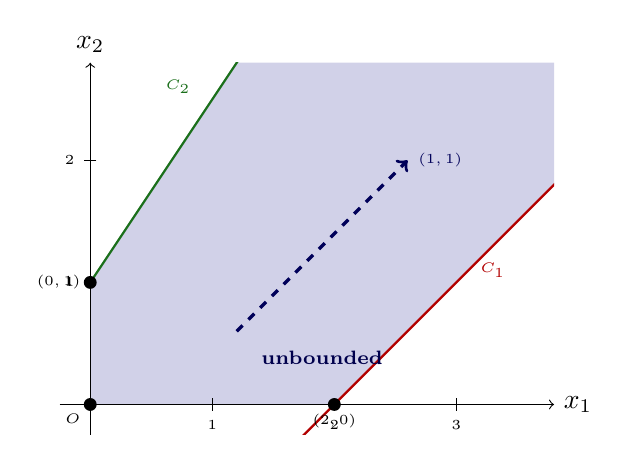
\begin{tikzpicture}[scale=1.55]
  % Feasible region clipped to box: C1 exits right at (3.8,1.8); C2 exits top at (1.2,2.8)
  \fill[NavyBlue!18](0,0)--(2,0)--(3.8,1.8)--(3.8,2.8)--(1.2,2.8)--(0,1)--cycle;
  \begin{scope}
    \clip (-0.25,-0.25) rectangle (3.8,2.8);
    \draw[red!70!black,thick](0,-2)--(6,4);
    \draw[ForestGreen!80!black,thick](0,1)--(2,4);
    \draw[->,NavyBlue!70!black,very thick,dashed](1.2,0.6)--(2.6,2.0)
        node[right,font=\tiny]{$(1,1)$};
  \end{scope}
  \draw[->](-0.25,0)--(3.8,0)node[right]{$x_1$};
  \draw[->](0,-0.25)--(0,2.8)node[above]{$x_2$};
  \foreach \x in {1,2,3}\draw(\x,.05)--(\x,-.05)node[below,font=\tiny]{$\x$};
  \foreach \y in {1,2}\draw(.05,\y)--(-.05,\y)node[left,font=\tiny]{$\y$};
  \fill(0,0)circle(1.5pt)node[below left,font=\tiny]{$O$};
  \fill(2,0)circle(1.5pt)node[below,font=\tiny]{$(2,0)$};
  \fill(0,1)circle(1.5pt)node[left,font=\tiny]{$(0,1)$};
  \node[red!70!black,font=\tiny]at(3.3,1.1){$C_1$};
  \node[ForestGreen!80!black,font=\tiny]at(0.72,2.6){$C_2$};
  \node[font=\scriptsize,NavyBlue!60!black]at(1.9,0.38){\textbf{unbounded}};
\end{tikzpicture}
\end{center}

\item Same feasible region as (iv). Every recession direction $d=(d_1,d_2)$ must satisfy
$d_2\ge d_1$ (from $C_1$), so $d_1-2d_2\le -d_1\le0$: the objective cannot grow along any
unbounded direction. Evaluating at the three vertices:
\[
  (0,0)\mapsto 0,\quad (2,0)\mapsto 2,\quad (0,1)\mapsto -2.
\]
Maximum $= \boldsymbol{2}$ at $(2,0)$ (\(\bigstar\)).

\begin{center}
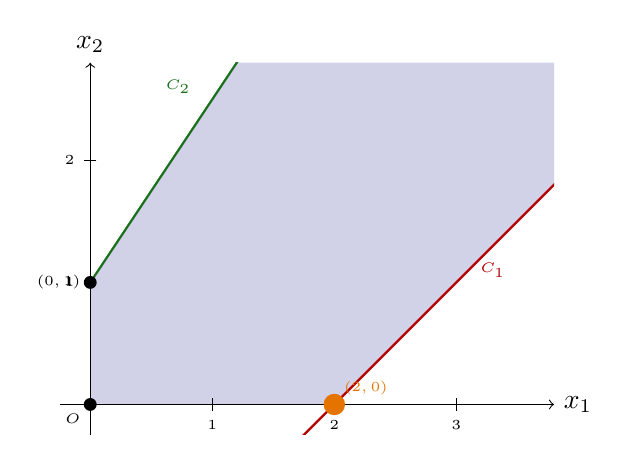
\begin{tikzpicture}[scale=1.55]
  \fill[NavyBlue!18](0,0)--(2,0)--(3.8,1.8)--(3.8,2.8)--(1.2,2.8)--(0,1)--cycle;
  \begin{scope}
    \clip (-0.25,-0.25) rectangle (3.8,2.8);
    \draw[red!70!black,thick](0,-2)--(6,4);
    \draw[ForestGreen!80!black,thick](0,1)--(2,4);
  \end{scope}
  \draw[->](-0.25,0)--(3.8,0)node[right]{$x_1$};
  \draw[->](0,-0.25)--(0,2.8)node[above]{$x_2$};
  \foreach \x in {1,2,3}\draw(\x,.05)--(\x,-.05)node[below,font=\tiny]{$\x$};
  \foreach \y in {1,2}\draw(.05,\y)--(-.05,\y)node[left,font=\tiny]{$\y$};
  \fill(0,0)circle(1.5pt)node[below left,font=\tiny]{$O$};
  \fill[orange!90!black](2,0)circle(2.5pt)
      node[above right,font=\tiny]{$(2,0)\;\bigstar$};
  \fill(0,1)circle(1.5pt)node[left,font=\tiny]{$(0,1)$};
  \node[red!70!black,font=\tiny]at(3.3,1.1){$C_1$};
  \node[ForestGreen!80!black,font=\tiny]at(0.72,2.6){$C_2$};
\end{tikzpicture}
\end{center}

\end{enumerate}
\end{explanation}

\paragraph{Different behavior:}
When solution exists:
\begin{enumerate}
    \item Could be unique
    \item Could have infinitely many solutions.
\end{enumerate}
If solution doesn't exists:
\begin{enumerate}[label=\arabic*., start=3]
    \item No part satisfies constraints. 
    \item Objective function is unbounded.
\end{enumerate}

\begin{definition}
    The feasible set/region is the set of values \(\vv{x}\) satisfying all the constraints. 
\end{definition}

\begin{remark}
    \quad 
    \begin{enumerate}
        \item Infeasible \(\iff \) feasible set \(= \varnothing\). 
        \item Unbounded implies feasible set being unbounded. (However, the reverse direction does not hold) 
        \item If feasible set is bounded and non-empty, then there is a solution. (comtinuous function on a compact domain attains a maximum)  
    \end{enumerate}
\end{remark}

\section{Deriving the general form of the (primal) linear program}

In general, if we have \(n\) variables \(x_1, x_2, \dots , x_n\). Our objective is to max/min \(\sum_{i=1}^n c_i x_i =  \vv{c}^T \vv{x} \) where \(\vv{c}\) is a vector of constants. 

Note that 
\[
    \min \vv{c}^T \vv{x} \iff \max - \vv{c}^T \vv{x} = (- \vv{c})^T \vv{x}.
\]
Thus, WLOG suppose we are maximizing. Now the constraints are  
\[
    a_{i1} x_1 + a_{i2} x_2 + \dots + a_{in} x_n \begin{Bmatrix}
        \le \\ = \\ \ge
    \end{Bmatrix} b_i,
\]
where \(a_{ij}, b_i\) are constants. Observe that 
\[
    \sum_{j} a_{ij} x_j = b_i \iff \sum_{j} a_{ij} x_j \le b_i \text{ and } \sum_{j} a_{ij} x_j \ge b_i,   
\]
and 
\[
    \sum_{j} a_{ij} x_j \ge b_i \iff \sum_{j} (-a_{ij}) x_j \le -b_i, 
\]
so we may assume \(\le\) always. 

Thus, the general form of the (primal) linear program is 
\[
    \begin{aligned}
        \max~ & \vv{c}^T \vv{x}  \\
           \text{subject to }  & A \vv{x} \le \vv{b}  \\
            & x_i \ge 0 \quad \forall i \in I \text{ for some } I \subseteq [n], 
    \end{aligned}
\]
where \(\vv{x} \in \mathbb{R} ^n\) are our variables, \(\vv{c} \in \mathbb{R} ^n\) is a constant vector of coefficients, \(\vv{b} \in \mathbb{R} ^m\) and \(A \in \mathbb{R} ^{m \times n}\) and we say \(\vv{y} \le \vv{z}\) iff \(y_i \le z_i\) for all \(i\).

\paragraph{Finding the solution}
Let \(v^*\) be the optimal value. Then for any feasible \(\vv{x}\) (i.e. \(A \vv{x} \le \vv{b}\)) we have \(\vv{c}^T \vv{x} \le v^*\).

\paragraph{Upper bounds in \(v^*\)}
\hfill \\
Idea: Take linear combination of the constraints to obtain upper bounds on the objective function.

\begin{eg}
\vphantom{d} \\
\begin{figure}[H]
    \centering
    \begin{tabular}{lcccc}
    \toprule
    & Beef (kg) & Noodles (kg) & Soup (kg) & \begin{tabular}[c]{@{}c@{}}Min. Daily\\ Requirement\end{tabular} \\ \midrule
    Vit A (mg/kg) & 35 & 0.5 & 0.5 & 0.5 mg \\
    Vit C (mg/kg) & 60 & 300 & 10 & 15 mg \\
    Fibre (g/kg)  & 30 & 20  & 10 & 4 g \\
    Cost (\$/kg)  & 75 & 50  & 15 & \\ \bottomrule
    \end{tabular}
\end{figure}

Now we want to minimize cost subject to each bowl provide the required Vit A, Vit C, Fibre. Now suppose \(x_B = \) kgs of beef, \(x_N = \) kgs of noodles, and \(x_S = \) kgs of soup. Then the problem can be formulated as 
\[
    \begin{aligned}
        \min~ & 75 x_B + 50 x_W + 15 x_S  \\
          \text{subject to }   & 35 x_B + 0.5 x_W + 0.5 x_S \ge 0.5  \\
            & 60 x_B + 300 x_W + 10 x_S \ge 15 \\
            & 30 x_B + 20 x_W + 10 x_S \ge 4 \\
            & x_B, x_N, x_W \ge 0.
    \end{aligned}
\]
Now observe that \(x_B = \frac{1}{10}, x_N = \frac{1}{20}, x_S = 0\) is feasible, so min cost \(\le 75 \cdot \frac{1}{10} + 50 \cdot \frac{1}{20} = 110\). 

Also, \(x_B \thickapprox 0.0095, x_N \thickapprox 0.038, x_S \thickapprox 0.290\) is feasible with cost \(\thickapprox \$ 7\).

We know that for any feasible solution, 
\[
    35 x_B + 0.5 x_N + 0.5 x_S \ge 0.5.
\]
Multiply it by \(\frac{75}{35}\), it becomes 
\[
    75 x_B + \frac{37.5}{35} x_N + \frac{37.5}{35} x_5 \ge \frac{37.5}{35}.
\] 
Note that the objective is 
\[
    75 x_B + 50 x_N + 15 x_S \ge 75 x_B + \frac{37.5}{35} x_N + \frac{37.5}{35} x_5 \ge \frac{37.5}{35}. 
\]
Using constraint 3:
\[
    30 x_B + 20 x_N + 10 x_S \ge 4,
\]
and multiply it by \(1.5\), we have 
\[
    45 x_B + 30 x_N + 15 x_S \ge 6,
\]
so the objective function 
\[
    75 x_B + 50 x_N + 15 x_S \ge 45 x_B + 30 x_N + 15 x_S \ge 6. 
\] 
Now note that
\[
     \text{objective} = \text{(constraint 1)} \times \frac{3120}{3758} + \text{(constraint 2)} \times \frac{274}{3758} + \text{(constraint 3)} \times \frac{5207}{3758} \ge 7.05,  
\]
which is the maximal lower bound. Now the problem is how we find these coefficients?
\end{eg}

\section{Dual Problem}
\begin{question}
    What is the optimal combination of the constraints to evaluate the best bound in the objective function?
\end{question}

If the problem is 
\[
    \begin{aligned}
        \max~ & c_1 x_1 + c_2 x_2 + \dots + c_n x_n  \\
            & a_{11} x_1 + a_{12} x_2 + \dots + a_{1n} x_n \le b_1  \\
            & a_{21} x_1 + a_{22} x_2 + \dots + a_{2n} x_n \le b_2 \\
            &\vdots \\
            & a_{m1} x_1 + a_{m2} x_2 + \dots + a_{mn} x_n \le b_m \\
            & x_1, \dots , x_s \ge 0, x_{s+1}, \dots , x_n \in \mathbb{R},
    \end{aligned}
\]
and we multiply the \(i\)-th constraint by \(\lambda _i\), then 
\[
    \left( \sum_{j=1}^m \lambda _j a_{j1}  \right) x_1 + \left( \sum_{j=1}^m \lambda _j a_{j2}  \right) x_2 + \dots + \left( \sum_{j=1}^m \lambda _j a_{jn}  \right) x_n \le \sum_{j=1}^m \lambda _j b_j.    
\]  
Our goal is to choose coefficients \(\lambda _j\) for \(j = 1, 2, \dots , m\) s.t. 
\begin{enumerate}
    \item we get an upper bound on the objective function 
    \item upper bound as small as possible.
\end{enumerate}  

We get a valid upper bound if 
\begin{enumerate}[(a)]
    \item When \(x_i \ge 0\), \(\sum_{j=1}^n \lambda _j a_{ji} \ge c_i \). 
    \item When \(x_i \in \mathbb{R} \), \(\sum_{j=1}^m \lambda _j a_{ji} = c_i \).    
\end{enumerate}

This is because if so, then 
\[
    \text{objective} \le \left( \sum_{j=1}^m \lambda _j a_{j1}  \right) x_1 + \left( \sum_{j=1}^m \lambda _j a_{j2}  \right) x_2 + \dots + \left( \sum_{j=1}^m \lambda _j a_{jn}  \right) x_n \le \sum_{j=1}^m \lambda _j b_j.
\]

Thus, we have the constraints 
\begin{itemize}
    \item for \(1 \le i \le s\), \(\sum_{j=1}^m a_{ji} \lambda _j \ge c_i \). 
    \item for \(s + 1 \le i \le n\), \(\sum_{j=1}^m a_{ji} \lambda _j = c_i \).  
\end{itemize}
Given this, we want to minimize \(\sum_{j=1}^m b_j \lambda _j \).

We call the primal program:
\[
    \begin{aligned}
        \max~ & \vv{c}^T \vv{x}  \\
            & A \vv{x} \le \vv{b}  \\
            & \vv{x} \ge \vv{0},
    \end{aligned}
\]
and the dual problem to be 
\[
    \begin{aligned}
        \min~ & \vv{b}^T \vv{\lambda }  \\
            & A^T \vv{\lambda } \ge \vv{c}^T  \\
            & \vv{\lambda } \ge 0 
    \end{aligned}
\]

\begin{remark}
    Note that the dual of the dual is the primal problem.
\end{remark}
\begin{proof}
Consider the primal problem
\[
(P)\qquad
\begin{aligned}
\max \;& c^T x\\
\text{s.t. }& Ax \le b,\\
& x \ge 0.
\end{aligned}
\]

Its dual is
\[
(D)\qquad
\begin{aligned}
\min \;& b^T y\\
\text{s.t. }& A^T y \ge c,\\
& y \ge 0.
\end{aligned}
\]

Rewrite $(D)$ as a maximization problem:
\[
(D)\iff
\begin{aligned}
\max\;& -b^T y\\
\text{s.t. }& -A^T y \le -c,\\
& y \ge 0.
\end{aligned}
\]

Applying the duality construction once more, the dual of $(D)$ is
\[
\begin{aligned}
\min\;& (-c)^T z\\
\text{s.t. }& (-A^T)^T z \ge -b,\\
& z \ge 0.
\end{aligned}
\]

Since $(-A^T)^T=-A$, this becomes
\[
\begin{aligned}
\min\;& -c^T z\\
\text{s.t. }& -Az \ge -b,\\
& z \ge 0.
\end{aligned}
\]

Equivalently,
\[
\begin{aligned}
\max\;& c^T z\\
\text{s.t. }& Az \le b,\\
& z \ge 0.
\end{aligned}
\]

This is exactly the primal problem $(P)$ (after renaming
the variable $z$ as $x$). Hence the dual of the dual is the primal.
\end{proof}

